\renewcommand{\theequation}{\theenumi}
\renewcommand{\thefigure}{\theenumi}

%\subsection{Independence}
\subsection{Using Definition}
\begin{enumerate}[label=\thesubsection.\arabic*.,ref=\thesubsection.\theenumi]
\numberwithin{equation}{enumi}
\numberwithin{figure}{enumi}

%
\item
Let $X_1 \sim  \gauss{0}{1}$ and $X_2 \sim  \gauss{0}{1}$. Plot the CDF and PDF of
%
\begin{equation}
V = X_1^2 + X_2^2 
\end{equation}
%
\solution The following codes
\begin{lstlisting}
codes/trans/6.1.1_CDF.py
codes/trans/6.1.1_PDf.py
\end{lstlisting}
generate the CDF of $V$  in Fig. \ref{fig:probman_trans_cdf_V} and the PDf of $V$ in Fig. \ref{fig:probman_trans_PDf_V} respectively.
\begin{figure}[!ht]
\centering
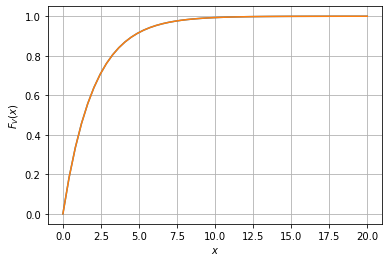
\includegraphics[width=\columnwidth]{figs/trans/6.1.1 cdf.png}
\caption{CDF of $V$}
\label{fig:probman_trans_cdf_V}
\end{figure}
%
\begin{figure}[!ht]
\centering
\includegraphics[width=\columnwidth]{figs/trans/6.1.1 PDf.png}
\caption{PDf of $V$}
\label{fig:probman_trans_PDf_V}
\end{figure}

\item
If
%
\begin{equation}
F_{V}(x) = 
\begin{cases}
1 - e^{-\alpha x} & x \geq 0 \\
0 & x < 0,
\end{cases}
\label{eq:probman_F_V_alpha}
\end{equation}
%
find $\alpha$.
\\
\solution For the value $\alpha=0.5$, the theory matches the simulation.  
The following code generates the CDF of $V$ in Fig. \ref{fig:probman_F_V_alpha} 
Fig. 
\begin{lstlisting}
codes/trans/6.1.2.py
\end{lstlisting}
%
\begin{figure}[!ht]
\centering
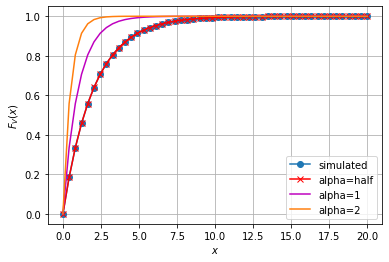
\includegraphics[width=\columnwidth]{figs/trans/6.1.2.png}
\caption{CDF of $V$}
\label{fig:probman_F_V_alpha}
\end{figure}
%
%
\item
\label{ch3_raleigh_sim}
Plot the CDF and PDf of
%
\begin{equation}
A = \sqrt{V}
\end{equation}
%
\solution The CDF and PDF of A are plotted in Figs. \ref{fig:probman_trans_cdf_A} and \ref{fig:probman_trans_PDf_A}
using the codes below.
\begin{lstlisting}
codes/trans/6.1.3_CDF.py
codes/trans/6.1.3_PDf.py
\end{lstlisting}

\begin{figure}[!ht]
\centering
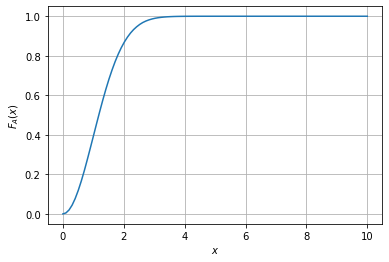
\includegraphics[width=\columnwidth]{figs/trans/6.1.3 cdf.png}
\caption{CDF of $A$}
\label{fig:probman_trans_cdf_A}
\end{figure}

\begin{figure}[!ht]
\centering
\includegraphics[width=\columnwidth]{figs/trans/6.1.3 PDf.png}
\caption{PDf of $V$}
\label{fig:probman_trans_PDf_A}
\end{figure}

%
\item
Find an expression for $F_{A}(x)$ using the definition. Plot this expression and compare with the result of problem \ref{ch3_raleigh_sim}. 
\\
\solution 
% Given,
% \begin{align}
% A = \sqrt{V}
% \end{align}

\begin{align} 
F_A(x) &= \pr{A \le x} = \pr{\sqrt{V} \le x}
\\
&= \pr{V \le x^2} = F_V\brak{x^2}
\end{align}
%
From \eqref{eq:probman_F_V_alpha}, 
\begin{align} 
F_V\brak{x^2} = 
\begin{cases}
1 - e^{-\alpha x^2} & x \geq 0 \\
0 & x < 0,
\end{cases}
\end{align}
%
Substituting 

\begin{align}
\alpha = \frac{1}{2}
\end{align}

%
\begin{align} 
F_V\brak{x^2} = 
\begin{cases}
1 - e^{- \frac{x^2}{2}} & x \geq 0 \\
0 & x < 0,
\end{cases}
\end{align}
%
The CDF of A is plotted in Fig. \ref{fig:probman_trans_cdf_A_theory} using the code below.
\begin{lstlisting}
codes/trans/6.1.4.py
\end{lstlisting}
%
\begin{figure}[!ht]
\centering
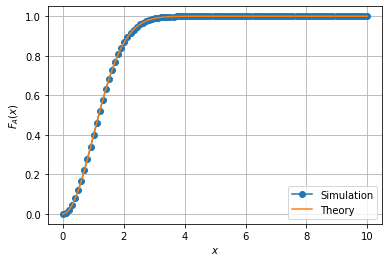
\includegraphics[width=\columnwidth]{figs/trans/6.1.4.png}
\caption{CDF of $A$}
\label{fig:probman_trans_cdf_A_theory}
\end{figure}
\item
Find an expression for $p_{A}(x)$.
\\
\solution
The PDf is obtained as
\begin{align}
f_V\brak{x^2} &= \frac{d}{dx}F_V\brak{x^2}
\\
&=
\begin{cases}
x e^{- \frac{x^2}{2}} & x \geq 0 \\
0 & x < 0,
\end{cases}
\end{align}
%
The PDf of A is plotted in \ref{fig:probman_trans_pdf_A_theory} using the code below.
\begin{lstlisting}
codes/trans/6.1.5.py
\end{lstlisting}
\begin{figure}[!ht]
\centering
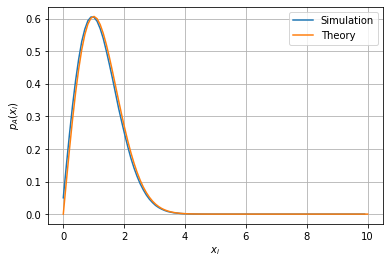
\includegraphics[width=\columnwidth]{figs/trans/6.1.5.png}
\caption{PDf of $A$}
\label{fig:probman_trans_pdf_A_theory}
\end{figure}
\end{enumerate}

%
\subsection{Using Jacobian}
%
\begin{enumerate}[label=\thesubsection.\arabic*.,ref=\thesubsection.\theenumi]
\numberwithin{equation}{enumi}
\numberwithin{figure}{enumi}

\item
Evaluate the joint PDF of $X_1,X_2$,  given by
%
\begin{equation}
p_{X_1,X_2}(x_1,x_2) = p_{X_1}\brak{x_1}p_{X_2}\brak{x_2}
\end{equation}
%
\solution From \eqref{eq:probman_gauss_pdf}
\begin{align}
p_{X_1}(x_1)&=\frac {1}{\sqrt {2\pi }}e^{-\frac {x_1^2}{2}}
\\
p_{X_2}(x_2)&=\frac {1}{\sqrt {2\pi }}e^{-\frac {x_2^2}{2}}
\\
\implies p_{X_1,X_2}(x_1,x_2) &= \frac {1}{\sqrt {2\pi }}e^{-\frac {x_1^2+x_2^2}{2}}
\label{eq:probman_pdf_x1x2}
\end{align}
 
%
\item
Let 
\begin{align}
 X_1 = \sqrt{V}\cos \theta
\\
 X_2 = \sqrt{V} \sin \theta.
\end{align}
Evaluate the Jacobian 
%
\begin{equation}
J =
\begin{vmatrix}
\frac{\partial x_1}{\partial v} & \frac{\partial x_2}{\partial v} \\
\frac{\partial x_1}{\partial \theta} & \frac{\partial x_2}{\partial \theta} 
\end{vmatrix}
\end{equation}
%
\solution
\begin{align}
J=\begin{vmatrix}
     \frac{1}{2\sqrt{v}}\cos\theta & \frac{1}{2\sqrt{v}}\sin\theta\\
       -v\sin\theta & v\cos\theta
\end{vmatrix}=\frac{1}{2}
\label{eq:probman_jacob_V}
\end{align}
\item
Find
%
\begin{equation}
p_{V,\Theta}\brak{v,\theta} = \abs{J}p_{X_1,X_2}\brak{x_1,x_2}
\end{equation}
%
\solution From \eqref{eq:probman_jacob_V} and \eqref{eq:probman_pdf_x1x2},
\begin{align}
p_{V,\Theta}\brak{v,\theta}=\frac{1}{4\pi}\exp\brak{-\frac{v}{2}}, v \ge 0, 0 < \theta < 2\pi
\label{eq:probman_pdf_V_theta}
\end{align}
%
\item
Find $p_{V}(v)$.
\\
\solution For $v \ge 0$, from \eqref{eq:probman_pdf_V_theta},
\begin{align}
p_{V}(v) &= \int_{0}^{2\pi} \frac{1}{4\pi}\exp\brak{-\frac{v}{2}} d \theta \\
&= \brak{2\pi} \times \frac{1}{4\pi}\exp\brak{-\frac{v}{2}} \\
&= \frac{1}{2}\exp\brak{-\frac{v}{2}}\\
\therefore p_{V}(v) &= 
\begin{cases}
\frac{1}{2}\exp\brak{-\frac{v}{2}} & v\geq 0 \\
0 & v< 0
\end{cases}
\label{eq:probman_pdf_V}
\end{align}
%

\item
Find $p_{\Theta}(\theta)$.  
\\
\solution For $0 \le \theta \le 2\pi$, from \eqref{eq:probman_pdf_V_theta},
\begin{align}
p_{\Theta}(\theta) &= \int_{0}^{\infty} \frac{1}{4\pi}\exp\brak{-\frac{v}{2}} d v \\
&= \frac{1}{2\pi} \left[1 - e^{-\frac{x}{2}} \right]_{0}^{\infty}\\
&= \frac{1}{2\pi}\\
\therefore p_{V}(v) &= 
\begin{cases}
\frac{1}{2\pi} & 0 \leq \theta \leq 2\pi \\
0 & \text{otherwise}
\end{cases}
\end{align}
%
\item
Are $V$ and $\Theta$ independent?
\\
\solution Yes,
\begin{align}
\because p_{V}(v)p_{\Theta}(\theta) &= \frac{1}{2}\exp\brak{-\frac{v}{2}} \times \frac{1}{2\pi}\\
&= \frac{1}{4\pi}\exp\brak{-\frac{v}{2}}\\
&= p_{V,\Theta}\brak{v,\theta}
\end{align}
\item
Find $p_{A}(x)$ using the Jacobian.
\\
\solution 
\begin{align}
p_{A}(x) &= \Pr(A=x) = \Pr(\sqrt{V} = x) \\
&= \Pr(V=x^2) = p_V(x^2)
\end{align}
From \eqref{eq:probman_pdf_V}, as $x^2 \ge 0$,
\begin{align}
p_{V}(x^2) &= \frac{1}{2}\exp\brak{-\frac{x^2}{2}} 
\end{align}
%%
% \item
% Find $p_{V}(v)$.  

% %
% %
% \item
% Find $p_{\Theta}(\theta)$.  

% %
% \item
% Are $Y$ and $\Theta$ independent?

% \item
% Find $p_{A}(x)$ using the Jacobian.

% %%
%\item
%Let $X_1 \sim  \gauss{2}{1}$ and $X_2 \sim  \gauss{3}{1}$. Find $E\sbrak{X_1X_2}$.  Try with different mean and variances. Comment.
%
%

%\section{The Transform Domain}
%\item
%Find the MGF of $X \sim \gauss{\mu}{\sigma^2}$. 
%
%\item
%Find the MGF of $Y$.
%
%%
%\item
%Find the PDF of $Y$ by inverting the MGF.
%
%%
\end{enumerate}
